\documentclass[11pt,letterpaper]{article}

\usepackage[margin=1in]{geometry}
\usepackage{enumitem}
\usepackage{hyperref}
\usepackage{amsmath}
\usepackage{booktabs}
\usepackage{float}
\usepackage{tikz}
\usetikzlibrary{decorations.pathmorphing, decorations.pathreplacing, calc, arrows.meta}

\title{16.07 Dynamics Problem Set 3}
\author{Due Wednesday, October 14}
\date{}

\begin{document}

\maketitle

\section*{Problem 1: Mass Properties of a T-Shaped Body}

\begin{figure}[h]
\centering
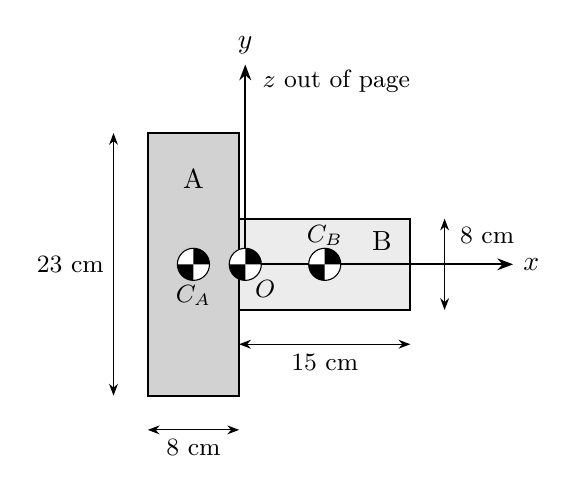
\begin{tikzpicture}[scale=1.45]
    % Units: 1 = 10 cm. Box A spans x in [-0.8,0], box B spans x in [0,1.5]; the T's CoM (body-frame origin O) is at (0.05395,0).
    \filldraw[fill=gray!35, draw=black, thick] (-0.8,-1.15) rectangle (0,1.15); % Box A (crossbar)
    \filldraw[fill=gray!15, draw=black, thick] (0,-0.4) rectangle (1.5,0.4);  % Box B (stem)

    % Box labels
    \node at (-0.4,0.75) {A};
    \node at (1.25,0.2) {B};

    % Body axes, with origin O at the CoM of the T-shaped body (z out of page)
    \draw[-{Stealth[length=2mm]}, thick] (0.05395,0) -- (2.4,0) node[right] {$x$};
    \draw[-{Stealth[length=2mm]}, thick] (0.05395,0) -- (0.05395,1.75) node[above] {$y$};
    \node[font=\small, anchor=west] at (0.12,1.6) {$z$ out of page};

    % CoM symbols: boxes A and B, and the T-shaped body (at O)
    \foreach \c in {-0.4, 0.05395, 0.75}{
        \filldraw[fill=white] (\c,0) circle (4pt);
        \fill (\c,0) -- ++(4pt,0) arc (0:90:4pt) -- cycle;
        \fill (\c,0) -- ++(-4pt,0) arc (180:270:4pt) -- cycle;
    }
    \node[below, font=\small] at (-0.4,-0.1) {$C_A$};
    \node[below right, font=\small] at (0.05395,-0.06) {$O$};
    \node[above, font=\small] at (0.75,0.08) {$C_B$};

    % Dimensions
    \draw[{Stealth[length=1.5mm]}-{Stealth[length=1.5mm]}] (-0.8,-1.45) -- (0,-1.45) node[midway, below, font=\small] {8 cm};
    \draw[{Stealth[length=1.5mm]}-{Stealth[length=1.5mm]}] (-1.1,-1.15) -- (-1.1,1.15) node[midway, left, font=\small] {23 cm};
    \draw[{Stealth[length=1.5mm]}-{Stealth[length=1.5mm]}] (0,-0.7) -- (1.5,-0.7) node[midway, below, font=\small] {15 cm};
    \draw[{Stealth[length=1.5mm]}-{Stealth[length=1.5mm]}] (1.8,-0.4) -- (1.8,0.4);
    \node[anchor=west, font=\small] at (1.85,0.25) {8 cm};
\end{tikzpicture}
\caption{Top view of the T-shaped body, made of box A (the crossbar) and box B (the stem). Both boxes are 5~cm thick in the $z$ direction, with their mid-planes at $z = 0$. The body-frame origin $O$ is at the center of mass of the T-shaped body, and $C_A$ and $C_B$ mark the centers of mass of the two boxes.}
\label{fig:tshape}
\end{figure}

\noindent The rigid T-shaped body in Fig.~\ref{fig:tshape} is made of two rectangular boxes. We'll describe it in the body frame shown, whose origin $O$ is at the center of mass of the T-shaped body: $x$ runs along the stem (the body's axis of symmetry), $y$ runs along the crossbar, and $z$ completes a right-handed frame, normal to the plane of the T. When the body lies flat, $z$ is vertical and rotation about $z$ is \emph{yaw}. We'll assume uniform density, so the centers of mass of the boxes, $C_A$ and $C_B$, are at their geometric centers. The mass, dimensions, and moments of inertia of each box are given in Table~\ref{tab:boxes}. Throughout this problem set, we'll work in centimeter--gram--second (CGS) units. Each box's moments of inertia are about its own center of mass, along axes parallel to the body frame, and each box's products of inertia about its own center of mass (i.e., the off-diagonal elements of the inertia matrix) are zero.

\begin{table}[H]
\centering
\small
\begin{tabular}{lccc}
\toprule
 & Mass & Dimensions $x\times y\times z$ & Moments of inertia about own CoM \\
Box & (g) & (cm) & $(J_{xx},\ J_{yy},\ J_{zz})$ ($10^{3}$~g\,cm$^2$) \\
\midrule
A (crossbar) & 588.8 & $8\times23\times5$ & $(27.18,\ \ 4.367,\ \ 29.10)$ \\
B (stem)     & 384.0 & $15\times8\times5$ & $(2.848,\ \ 8.000,\ \ 9.248)$ \\
\bottomrule
\end{tabular}
\caption{Mass properties of the two boxes. Moments of inertia are about each box's own CoM, along axes parallel to the body frame.}
\label{tab:boxes}
\end{table}

\begin{enumerate}[label=(\alph*)]
    \item \textbf{Mass:} Find the total mass $m$ of the T-shaped body.

    \item \textbf{Center of mass:} Find the position vectors $\mathbf{r}_1$ and $\mathbf{r}_2$ from the center of mass $O$ of the T-shaped body to the box centers of mass $C_A$ and $C_B$, respectively, expressed in the body frame. (You'll first need to locate $O$.)

    \item \textbf{Inertia matrix:} Using $\mathbf{r}_1$, $\mathbf{r}_2$, and the parallel axis theorem, find the inertia matrix $\mathbf{J}$ of the T-shaped body about its center of mass $O$, expressed in the body frame.
\end{enumerate}

\section*{Problem 2: The Bifilar Pendulum}

\begin{figure}[h]
\centering
% ---------------- Left panel: oblique view of the suspended T-shaped body ----------------
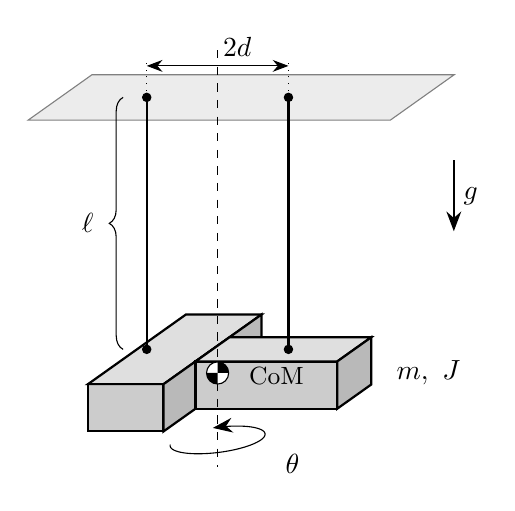
\begin{tikzpicture}[scale=1.0,
    x={(1cm,0cm)}, y={(0.45cm,0.32cm)}, z={(0cm,1cm)}]
    % 3D coordinates (x,y,z); z is up, x along the stem, origin directly above the body's CoM.
    % Drawing scale: 1 unit = 1/12 m, so d = 7.5 cm -> 0.9 units.
    \def\hd{0.9}    % d, half of the string separation
    \def\Ls{3.2}    % string length \ell (not to scale)
    \def\bh{0.6}    % body thickness (5 cm)
    \def\zt{-\Ls}           % top surface of the body
    \def\zb{-\Ls-\bh}       % bottom surface of the body

    % Ceiling
    \filldraw[fill=gray!15, draw=gray] (-2.0,-0.9,0) -- (2.6,-0.9,0) -- (2.6,0.9,0) -- (-2.0,0.9,0) -- cycle;

    % Box A (crossbar): x in [-1.0247,-0.0647], y in [-1.38,1.38]
    \filldraw[fill=gray!40, draw=black, thick]
        (-1.0247,-1.38,\zt) -- (-0.0647,-1.38,\zt) -- (-0.0647,-1.38,{\zb}) -- (-1.0247,-1.38,{\zb}) -- cycle;
    \filldraw[fill=gray!25, draw=black, thick]
        (-1.0247,-1.38,\zt) -- (-0.0647,-1.38,\zt) -- (-0.0647,1.38,\zt) -- (-1.0247,1.38,\zt) -- cycle;
    \filldraw[fill=gray!55, draw=black, thick]
        (-0.0647,-1.38,\zt) -- (-0.0647,1.38,\zt) -- (-0.0647,1.38,{\zb}) -- (-0.0647,-1.38,{\zb}) -- cycle;

    % Box B (stem): x in [-0.0647,1.7353], y in [-0.48,0.48]
    \filldraw[fill=gray!40, draw=black, thick]
        (-0.0647,-0.48,\zt) -- (1.7353,-0.48,\zt) -- (1.7353,-0.48,{\zb}) -- (-0.0647,-0.48,{\zb}) -- cycle;
    \filldraw[fill=gray!25, draw=black, thick]
        (-0.0647,-0.48,\zt) -- (1.7353,-0.48,\zt) -- (1.7353,0.48,\zt) -- (-0.0647,0.48,\zt) -- cycle;
    \filldraw[fill=gray!55, draw=black, thick]
        (1.7353,-0.48,\zt) -- (1.7353,0.48,\zt) -- (1.7353,0.48,{\zb}) -- (1.7353,-0.48,{\zb}) -- cycle;

    % Vertical axis through the CoM
    \draw[dashed] (0,0,0.6) -- (0,0,{\zb-0.9});

    % Strings
    \draw[thick] (-\hd,0,0) -- (-\hd,0,\zt);
    \draw[thick] (\hd,0,0) -- (\hd,0,\zt);
    \filldraw (-\hd,0,0) circle (1.5pt);
    \filldraw (\hd,0,0) circle (1.5pt);
    \filldraw (-\hd,0,\zt) circle (1.5pt);
    \filldraw (\hd,0,\zt) circle (1.5pt);

    % CoM marker (directly below the midpoint between the strings)
    \coordinate (CM) at (0,0,{-\Ls-\bh/2});
    \filldraw[fill=white] (CM) circle (4pt);
    \fill (CM) -- ++(4pt,0) arc (0:90:4pt) -- cycle;
    \fill (CM) -- ++(-4pt,0) arc (180:270:4pt) -- cycle;
    \node[font=\small, right] at ($(CM)+(0.32,-0.1)$) {CoM};

    % Separation 2d (dimension line above the ceiling)
    \draw[dotted] (-\hd,0,0) -- (-\hd,0,0.5);
    \draw[dotted] (\hd,0,0) -- (\hd,0,0.5);
    \draw[{Stealth[length=2mm]}-{Stealth[length=2mm]}] (-\hd,0,0.4) -- (\hd,0,0.4);
    \node[above] at (0.25,0,0.4) {$2d$};

    % String length \ell (brace to the left of the left string)
    \draw[decorate, decoration={brace, amplitude=5pt}]
        (-\hd-0.3,0,\zt) -- (-\hd-0.3,0,0);
    \node at (-\hd-0.75,0,{-\Ls/2}) {$\ell$};

    % Mass and inertia label
    \node[right] at (2.15,0,{-\Ls-\bh/2}) {$m,\ J$};

    % Twist angle about the vertical axis
    \draw[-{Stealth[length=2.5mm]}] plot[domain=200:480, samples=80, variable=\t]
        ({0.55*cos(\t)},{0.55*sin(\t)},{\zb-0.55});
    \node at (0.95,0,{\zb-0.85}) {$\theta$};

    % Gravity
    \draw[-{Stealth[length=2.5mm]}, thick] (3.0,0,-0.8) -- (3.0,0,-1.7);
    \node[right] at (3.0,0,-1.25) {$g$};
\end{tikzpicture}
\hspace{0.3cm}
% ---------------- Right panel: top view with the body twisted ----------------
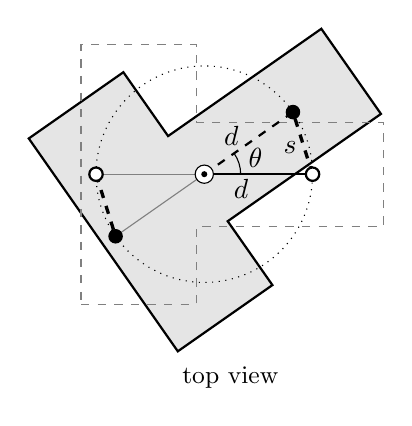
\begin{tikzpicture}[scale=1.1]
    % Drawing scale: d = 7.5 cm -> 1.25 units; the T outline is compressed to fit (not to scale). Origin at the body's CoM.
    \def\hd{1.25}   % d
    \def\th{35}     % twist angle shown
    \def\tshape{(-1.4232,-1.5) -- (-0.0899,-1.5) -- (-0.0899,-0.6) -- (2.07,-0.6) -- (2.07,0.6) -- (-0.0899,0.6) -- (-0.0899,1.5) -- (-1.4232,1.5) -- cycle} % T outline, compressed (not to scale)

    % Twisted body
    \begin{scope}[rotate=\th]
        \filldraw[fill=gray!20, draw=black, thick] \tshape;
    \end{scope}

    % Body outline at equilibrium
    \draw[dashed, gray] \tshape;

    % Circle of radius d traced by the body's string attachment points
    \draw[dotted] (0,0) circle (\hd);

    % Radii of length d: at rest (to the ceiling attachment) and twisted (to the body attachment)
    \draw[thick] (0,0) -- (\hd,0);
    \draw[thick, dashed] (0,0) -- ({\hd*cos(\th)},{\hd*sin(\th)});
    \draw[gray] (0,0) -- (-\hd,0);
    \draw[gray] (0,0) -- ({-\hd*cos(\th)},{-\hd*sin(\th)});

    % Horizontal projections of the strings (length s)
    \draw[very thick, dashed] (\hd,0) -- ({\hd*cos(\th)},{\hd*sin(\th)});
    \draw[very thick, dashed] (-\hd,0) -- ({-\hd*cos(\th)},{-\hd*sin(\th)});

    % Attachment points: open = ceiling (fixed), filled = body
    \filldraw[fill=white, thick] (\hd,0) circle (2.2pt);
    \filldraw[fill=white, thick] (-\hd,0) circle (2.2pt);
    \filldraw ({\hd*cos(\th)},{\hd*sin(\th)}) circle (2.2pt);
    \filldraw ({-\hd*cos(\th)},{-\hd*sin(\th)}) circle (2.2pt);

    % Labels for the d--d--s triangle
    \node[below, inner sep=1pt] at ({\hd/2-0.2},-0.02) {$d$};
    \node at ({0.55*\hd*cos(\th)-0.25},{0.55*\hd*sin(\th)+0.05}) {$d$};
    \node[inner sep=1.5pt] at ({\hd*cos(\th/2)-0.2},{\hd*sin(\th/2)-0.07}) {$s$};

    % Twist angle
    \draw (0.42,0) arc (0:\th:0.42);
    \node at ({0.62*cos(\th/2)},{0.62*sin(\th/2)}) {$\theta$};

    % Vertical axis (out of the page) through the CoM
    \filldraw[fill=white] (0,0) circle (3pt);
    \fill (0,0) circle (1pt);

    \node[font=\small] at (0.3,-2.35) {top view};
\end{tikzpicture}
\caption{The T-shaped body from Problem 1 hung as a bifilar pendulum. Left: oblique view at rest; the strings attach to the top of the body on its $x$ axis, a distance $d$ on either side of the CoM. Right: top view with the body twisted by $\theta$ about the vertical axis through its center of mass (pointing out of the page). Open circles mark where the strings attach to the ceiling (fixed); filled circles mark where they attach to the body. The thick dashed segments of length $s$ are the horizontal projections of the strings. Drawings are not to scale.}
\label{fig:bifilar}
\end{figure}

\noindent A bifilar (``two-string'') pendulum is a classic technique for measuring the moment of inertia of an object. Early NACA engineers used it to measure the yaw moment of inertia of full-scale airplanes, and it is still widely used today for drones, small satellites, and aircraft components. In this problem, you'll derive the equation of motion for a general bifilar pendulum, then use the T-shaped body from Problem 1 as a working example.

A rigid body of mass $m$ is suspended from the ceiling by two massless, inextensible strings, each of length $\ell$. The strings attach to the ceiling at two points a horizontal distance $2d$ apart, and to the body at two points that are also $2d$ apart, so the strings hang vertical and parallel at rest. The body hangs with its center of mass (CoM) directly below the midpoint between the strings, as shown in Fig.~\ref{fig:bifilar}. In our working example, the T-shaped body hangs flat, with its body $z$ axis vertical, and the strings attach to its top surface at two points on its $x$ axis, a distance $d$ on either side of its CoM. Let $J$ be the (unknown) moment of inertia of the body about the vertical axis through its CoM, and let $\theta$ be the angle the body is twisted about that axis, measured from its rest position.

When the body is twisted, the strings tilt and the body must rise slightly, so gravity provides a restoring torque. By measuring the period of small twisting oscillations, we can infer $J$. We'll make the following assumptions throughout this problem:
\begin{itemize}
    \item The system is frictionless, and air resistance is negligible.
    \item The strings remain taut at all times.
    \item The body only twists: its CoM stays on the vertical axis (no side-to-side swinging) and the body stays level. The system then has a single generalized coordinate, $\theta$, and the height of the body is determined by $\theta$ through the string-length constraint.
\end{itemize}
We'll use $T$ for kinetic energy, $U$ for potential energy, $\mathcal{L} = T - U$ for the Lagrangian, and $P$ for the period of oscillation.

\subsection*{Equations of Motion}

\begin{enumerate}[label=(\alph*)]
    \item \textbf{Geometry and energies:} Using the top view in Fig.~\ref{fig:bifilar}, find the horizontal displacement $s$ between the top and bottom ends of each string as a function of $d$ and $\theta$. Then use the fixed string length to find the vertical displacement $h(\theta)$ of the body. Write the kinetic energy $T$ (including both the rotation of the body about the vertical axis and the vertical translation of its CoM) and the gravitational potential energy $U$, and combine them to obtain the Lagrangian $\mathcal{L}(\theta,\dot\theta)$.

    \item \textbf{Small-angle expansion:} Taylor expand the Lagrangian to \emph{second order} in the small quantities $\theta$ and $\dot\theta$ about the equilibrium $\theta=\dot\theta=0$. Which terms survive? Explain why the kinetic energy of the body's vertical translation no longer appears.

    \item \textbf{Linearized equation of motion:} Apply the Euler--Lagrange equation to your quadratic Lagrangian to derive the linearized equation of motion, and write it in the standard form
    \[
    \ddot\theta + \omega^2\,\theta = 0 .
    \]

    \item \textbf{Natural frequency and period:} Write the natural frequency $\omega$ (in rad/s) and the period $P$ (in seconds) of small oscillations in terms of $m$, $g$, $d$, $\ell$, and $J$.

    \item \textbf{Measuring the inertia:} Solve your result from part (d) for the moment of inertia $J$ as a function of the measured period $P$ and the other system parameters.

\end{enumerate}

\subsection*{Error Analysis}

Suppose you use this setup to measure the yaw moment of inertia of the T-shaped body. You measure the string separation $2d$ and the string length $\ell$ with a ruler to within about $\pm 0.1$~cm, and you may assume $m$ and $g$ are known precisely enough that their errors are negligible. You time the oscillations with a hand-held stopwatch, which (because of your reaction time) gives an uncertainty of about $\pm 0.1$~s on each timed interval, regardless of how long the interval is. Use the nominal values $\ell = 200$~cm and $2d = 15$~cm. Denote the uncertainty in a quantity $x$ by $\sigma_x$ (e.g., $\sigma_\ell = 0.1$~cm, and since $d$ is half the measured separation, $\sigma_d = 0.05$~cm).

\begin{enumerate}[label=(\alph*)]
\setcounter{enumi}{5}
	\item \textbf{Nominal period:} Using your values of $m$ and $J = J_{zz}$ from Problem 1 and $g = 981$~cm/s$^2$, compute the natural frequency $\omega$ and the period $P$ you would expect to measure.

    \item \textbf{Error propagation:} For small errors, we can calculate the expected error in the output of a function by mapping the expected errors in the inputs through the function's derivative. If the error sources are independent, then we can combine them by adding them in quadrature (i.e., taking the root-sum-square, or RSS). For a function $z = f(x,y)$, we would have:
    	\begin{equation*}
    		\sigma_z = \sqrt{\left( \frac{\partial f}{\partial x} \sigma_x \right)^2+ \left( \frac{\partial f}{\partial y} \sigma_y \right)^2}
    	\end{equation*} 
     Using your expression for $J$ from (e), derive an expression for the uncertainty $\sigma_J$ in terms of the uncertainties $\sigma_d$, $\sigma_\ell$, and $\sigma_P$. Assume the measurement errors are independent.

    \item \textbf{Timing a single period:} Suppose you time a single oscillation. Compute the contribution of each measurement to $\sigma_J$, as well as the total fractional uncertainty $\sigma_J/J$ expressed as a percentage. What is the dominant source of error?

    \item \textbf{Timing 10 periods:} Now suppose you instead time 10 consecutive oscillations with the same stopwatch (so the total time is still uncertain by $\pm 0.1$~s) and divide by 10 to get $P$. Find the resulting uncertainty in $P$ and repeat your analysis from part (h). Has the dominant source of error changed?

\end{enumerate}

\end{document}
